\documentclass[border=10pt]{standalone}
\usepackage[utf8]{inputenc}
\usepackage[T1]{fontenc}
\usepackage{tikz}
\usetikzlibrary{positioning,fit,backgrounds,arrows.meta,calc}

\pgfdeclarelayer{lTest}
\pgfdeclarelayer{lEnv}
\pgfdeclarelayer{lAgent}
\pgfsetlayers{lTest,lEnv,lAgent,main}

\begin{document}
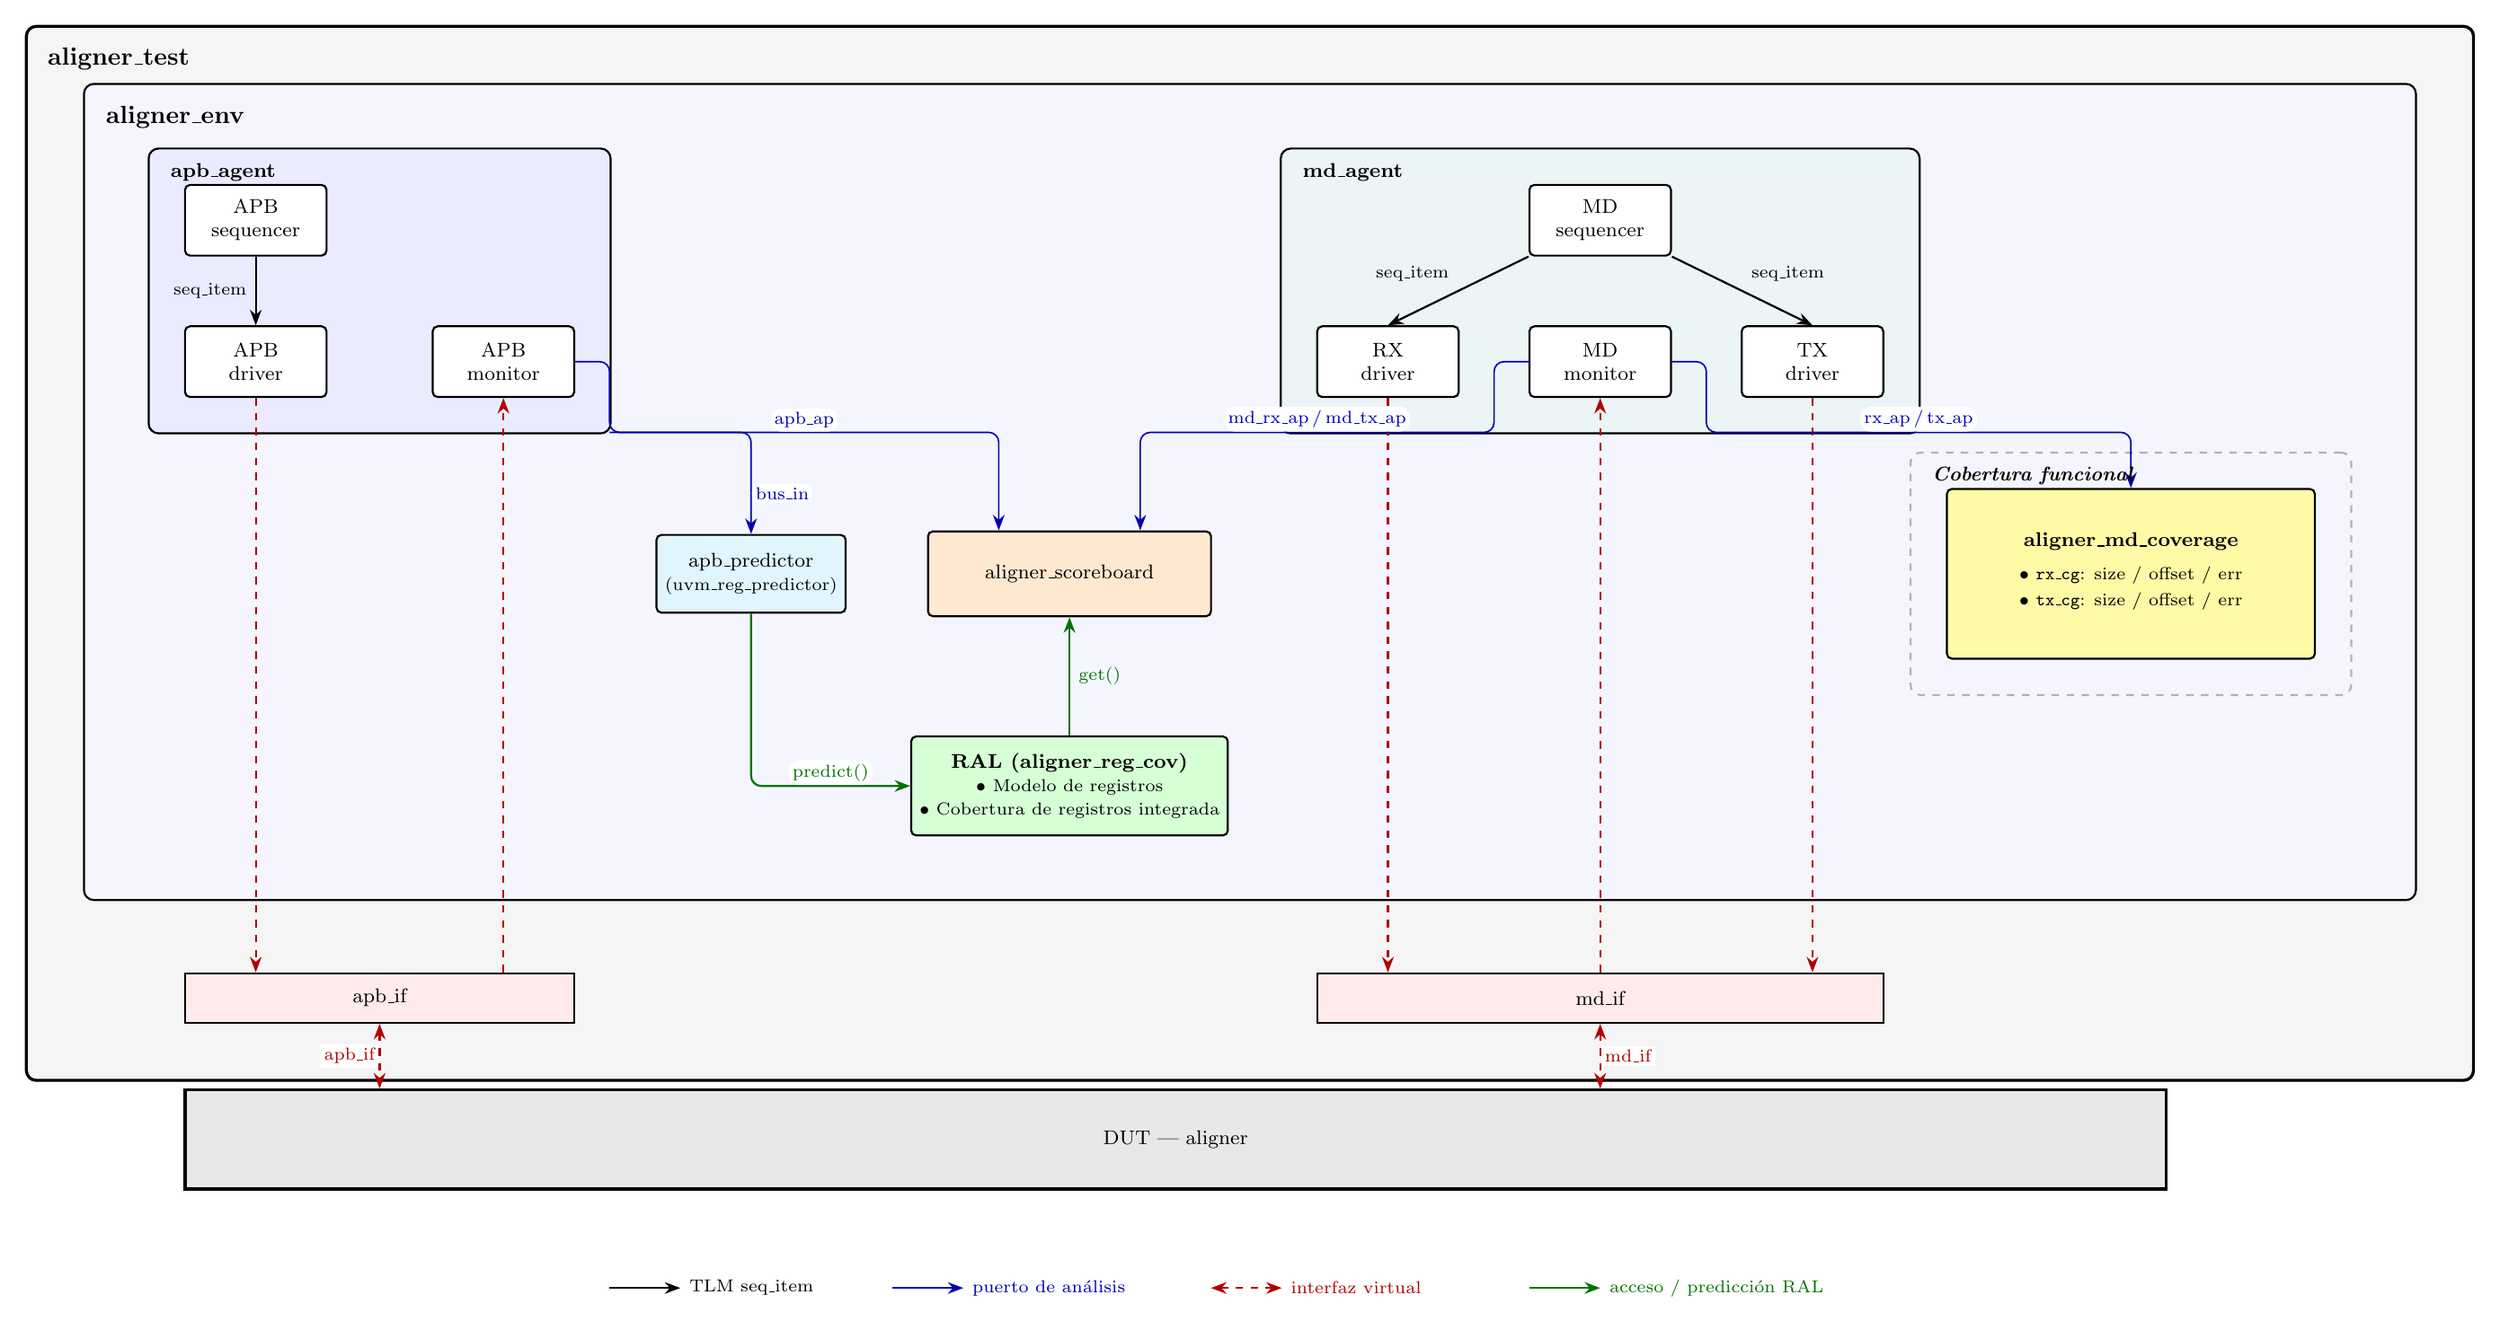
\begin{tikzpicture}[
  font=\footnotesize,
  comp/.style={draw,thick,rounded corners=2pt,fill=white,
    minimum width=20mm,minimum height=10mm,align=center},
  ifc/.style={draw,thick,fill=red!8,minimum height=7mm,align=center},
  scb/.style={draw,thick,rounded corners=2pt,fill=orange!18,
    minimum width=40mm,minimum height=12mm,align=center},
  pred/.style={draw,thick,rounded corners=2pt,fill=cyan!12,
    minimum width=26mm,minimum height=11mm,align=center},
  cov/.style={draw,thick,rounded corners=2pt,fill=yellow!35,
    minimum width=52mm,minimum height=24mm,align=center},
  ral/.style={draw,thick,rounded corners=2pt,fill=green!16,
    minimum width=44mm,minimum height=14mm,align=center},
  dut/.style={draw,very thick,fill=gray!18,
    minimum width=280mm,minimum height=14mm,align=center},
  tlm/.style={-{Stealth[length=2.2mm]},thick},
  ana/.style={-{Stealth[length=2.2mm]},semithick,blue!70!black},
  vif/.style={-{Stealth[length=2.2mm]},thick,dashed,red!70!black},
  vifb/.style={{Stealth[length=2.2mm]}-{Stealth[length=2.2mm]},thick,dashed,red!70!black},
  ralw/.style={-{Stealth[length=2.2mm]},thick,green!45!black},
  lbl/.style={fill=white,inner sep=1.5pt,font=\scriptsize},
]

% ============================================================
% 1. POSICIONAMIENTO DE BLOQUES (X-Y Exactos sin superposición)
% ============================================================

% -- APB Agent --
\node[comp] (apbseqr) at (1.0, 14.5) {APB\\sequencer};
\node[comp] (apbdrv)  at (1.0, 12.5) {APB\\driver};
\node[comp] (apbmon)  at (4.5, 12.5) {APB\\monitor};

% -- Predictor explícito --
\node[pred] (apb_predictor) at (8.0, 9.5) {apb\_predictor\\{\scriptsize (uvm\_reg\_predictor)}};

% -- Componentes Centrales del ENV --
\node[scb]  (scb)  at (12.5, 9.5) {aligner\_scoreboard};
\node[ral]  (ral)  at (12.5, 6.5) {
  \textbf{RAL (aligner\_reg\_cov)}\\
  {\scriptsize $\bullet$ Modelo de registros}\\
  {\scriptsize $\bullet$ Cobertura de registros integrada}
};

% -- MD Agent --
\node[comp] (mdseqr)  at (20.0, 14.5) {MD\\sequencer};
\node[comp] (mdrx)    at (17.0, 12.5) {RX\\driver};
\node[comp] (mdmon)   at (20.0, 12.5) {MD\\monitor};
\node[comp] (mdtx)    at (23.0, 12.5) {TX\\driver};

% -- Cobertura MD --
\node[cov] (mdcov) at (27.5, 9.5) {
  \textbf{aligner\_md\_coverage}\\[4pt]
  \begin{tabular}{@{}l@{}}
    \scriptsize $\bullet$ \texttt{rx\_cg}: size / offset / err\\[1pt]
    \scriptsize $\bullet$ \texttt{tx\_cg}: size / offset / err\\[1pt]
  \end{tabular}
};

% -- Interfaces y DUT --
\node[ifc,minimum width=55mm]  (apbif) at (2.75, 3.5) {apb\_if};
\node[ifc,minimum width=80mm]  (mdif)  at (20.0, 3.5) {md\_if};
\node[dut] (dut) at (14.0, 1.5) {DUT — aligner};


% ============================================================
% 2. CONEXIONES TLM (Secuenciadores a Drivers)
% ============================================================
\draw[tlm] (apbseqr) -- (apbdrv) node[midway,left,font=\scriptsize]{seq\_item};

% MD Sequencer conecta a ambos drivers limpiamente sin tocar el monitor
\draw[tlm] (mdseqr.south west) -- (mdrx.north) node[midway,above left,font=\scriptsize]{seq\_item};
\draw[tlm] (mdseqr.south east) -- (mdtx.north) node[midway,above right,font=\scriptsize]{seq\_item};


% ============================================================
% 3. INTERFACES VIRTUALES (Rutas verticales directas hacia abajo)
% ============================================================
\draw[vif] (apbdrv.south) -- (apbdrv|-apbif.north);
\draw[vif] (apbmon|-apbif.north) -- (apbmon.south);
\draw[vifb](apbif.south) -- (apbif.south|-dut.north) node[midway,lbl,left]{apb\_if};

\draw[vif] (mdrx.south)  -- (mdrx|-mdif.north);
\draw[vif] (mdtx.south)  -- (mdtx|-mdif.north);
\draw[vif] (mdmon|-mdif.north) -- (mdmon.south);
\draw[vifb](mdif.south) -- (mdif.south|-dut.north) node[midway,lbl,right]{md\_if};


% ============================================================
% 4. PUERTOS DE ANÁLISIS (Rutas aisladas con esquinas curvas)
% ============================================================

% --- APB Monitor -> Predictor y Scoreboard ---
% Bajan al corredor vacío en Y=11.5 y se distribuyen.
\draw[ana, rounded corners=4pt] (apbmon.east) 
    -- (6.0, 12.5) -- (6.0, 11.5) -- (8.0, 11.5) 
    -- (apb_predictor.north) node[pos=0.6, lbl, right] {bus\_in};

\draw[ana, rounded corners=4pt] (6.0, 11.5) 
    -- (11.5, 11.5) node[midway, lbl, above] {apb\_ap} 
    -- ($(scb.north) - (10mm,0)$);


% --- MD Monitor -> Scoreboard ---
% Sale por la izquierda, baja al corredor Y=11.5 y conecta.
\draw[ana, rounded corners=4pt] (mdmon.west) 
    -- (18.5, 12.5) -- (18.5, 11.5) 
    -- (13.5, 11.5) node[midway, lbl, above] {\scriptsize md\_rx\_ap\,/\,md\_tx\_ap} 
    -- ($(scb.north) + (10mm,0)$);


% --- MD Monitor -> MD Coverage ---
% Sale por la derecha, baja al corredor Y=11.5 y conecta.
\draw[ana, rounded corners=4pt] (mdmon.east) 
    -- (21.5, 12.5) -- (21.5, 11.5) 
    -- (27.5, 11.5) node[midway, lbl, above] {rx\_ap\,/\,tx\_ap} 
    -- (mdcov.north);


% ============================================================
% 5. CONEXIONES DEL RAL (Limpias y directas)
% ============================================================
\draw[ralw, rounded corners=4pt] (apb_predictor.south) |- (ral.west) 
    node[pos=0.75, lbl, above] {predict()};

\draw[ralw] (ral.north) -- (scb.south) 
    node[midway, right, font=\scriptsize] {get()};


% ============================================================
% 6. CAJAS CONTENEDORAS (Fondos)
% ============================================================
\begin{pgfonlayer}{lAgent}
  \node[draw,thick,rounded corners,fill=blue!8,inner sep=5mm,
        fit=(apbseqr)(apbdrv)(apbmon)] (apbbox) {};
        
  \node[draw,thick,rounded corners,fill=teal!8,inner sep=5mm,
        fit=(mdseqr)(mdrx)(mdmon)(mdtx)] (mdbox) {};
        
  \node[draw=gray!60, dashed, thick, rounded corners, inner sep=5mm,
        fit=(mdcov)] (covbox) {};
\end{pgfonlayer}

\begin{pgfonlayer}{lEnv}
  \node[draw,thick,rounded corners,fill=blue!4,inner sep=9mm,
        fit=(apbbox)(mdbox)(scb)(ral)(covbox)(apb_predictor)] (envbox) {};
\end{pgfonlayer}

\begin{pgfonlayer}{lTest}
  \node[draw,very thick,rounded corners,fill=black!4,inner sep=8mm,
        fit=(envbox)(apbif)(mdif)] (testbox) {};
\end{pgfonlayer}


% ============================================================
% 7. ETIQUETAS DE CAJAS
% ============================================================
\node[anchor=north west,font=\bfseries,xshift=2mm,yshift=-2mm]
    at (testbox.north west) {aligner\_test};
\node[anchor=north west,font=\bfseries,xshift=2mm,yshift=-2mm]
    at (envbox.north west)  {aligner\_env};
\node[anchor=north west,font=\bfseries\footnotesize,xshift=2mm,yshift=-1mm]
    at (apbbox.north west)  {apb\_agent};
\node[anchor=north west,font=\bfseries\footnotesize,xshift=2mm,yshift=-1mm]
    at (mdbox.north west)   {md\_agent};
\node[anchor=north west,font=\bfseries\footnotesize\itshape,xshift=2mm,yshift=-1mm]
    at (covbox.north west)  {Cobertura funcional};


% ============================================================
% 8. LEYENDA (Re-centrada)
% ============================================================
\begin{scope}[shift={(6.0, -0.6)}]
  \draw[tlm]  (0,0)    -- ++(1.0,0) node[right,font=\scriptsize]{TLM seq\_item};
  \draw[ana]  (4.0,0)  -- ++(1.0,0) node[right,font=\scriptsize]{puerto de análisis};
  \draw[vifb] (8.5,0)  -- ++(1.0,0) node[right,font=\scriptsize]{interfaz virtual};
  \draw[ralw] (13.0,0) -- ++(1.0,0) node[right,font=\scriptsize]{acceso / predicción RAL};
\end{scope}

\end{tikzpicture}
\end{document}